% Asset ID: FA22CentreOfMassTikZ-001
% Source: Phase 4 generated TikZ asset for FA22 Centre of Mass
% Related lesson section: Section 9 TikZ placeholders
% Purpose: Particles on a line worked example.
\documentclass[tikz,border=8pt]{standalone}
\usepackage{amsmath}
\definecolor{Canvas}{HTML}{FAF9F6}
\definecolor{Ink}{HTML}{2C2C2E}
\definecolor{LineSoft}{HTML}{E5E5EA}
\definecolor{Gold}{HTML}{D4AF37}
\definecolor{Accent}{HTML}{C5A059}
\definecolor{Blush}{HTML}{FBEFEF}
\begin{document}
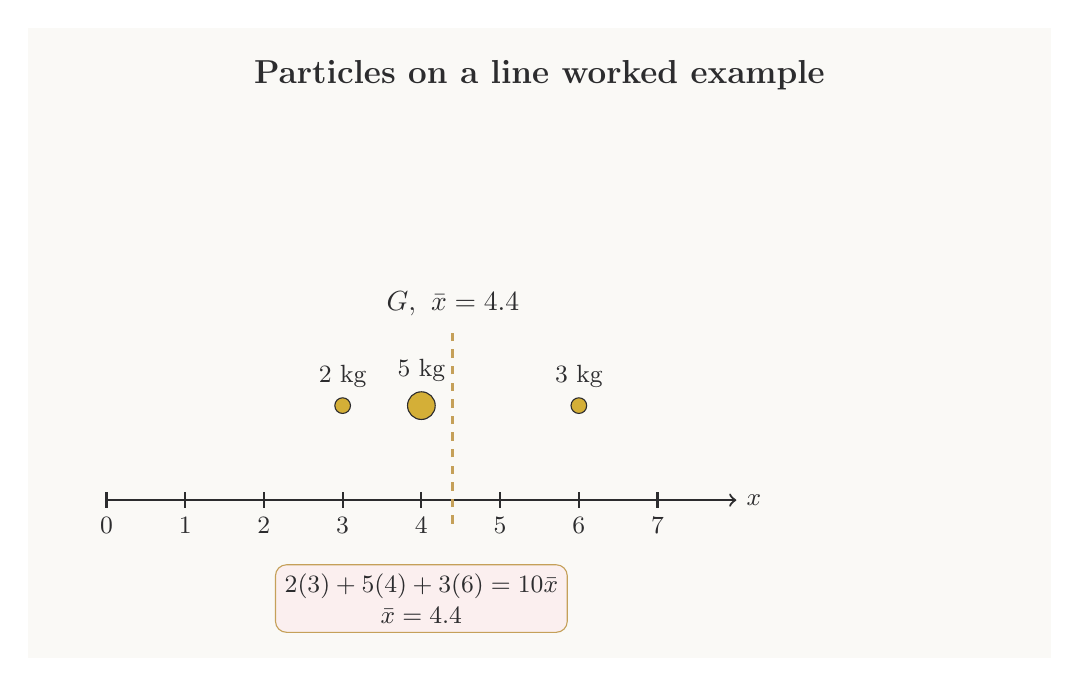
\begin{tikzpicture}[every node/.style={font=\small,text=Ink},line/.style={draw=Ink,line width=0.8pt},gold/.style={draw=Accent,line width=1.1pt},dot/.style={circle,fill=Gold,draw=Ink,inner sep=2pt}]
\fill[Canvas] (-1,-1) rectangle (12,7);
\node[font=\bfseries\large] at (5.5,6.4) {Particles on a line worked example};

\draw[line,->] (0,1) -- (8,1) node[right] {$x$};
\foreach \x in {0,...,7}{\draw[line] (\x,0.9)--(\x,1.1);\node[below] at (\x,0.9){$\x$};}
\node[dot,label=above:{$2\text{ kg}$}] at (3,2.2){};
\node[dot,minimum size=10pt,label=above:{$5\text{ kg}$}] at (4,2.2){};
\node[dot,label=above:{$3\text{ kg}$}] at (6,2.2){};
\draw[gold,dashed] (4.4,0.7)--(4.4,3.2);\node[font=\bfseries] at (4.4,3.5){$G,\ \bar{x}=4.4$};
\node[draw=Accent,fill=Blush,rounded corners,align=center] at (4,-0.25){$2(3)+5(4)+3(6)=10\bar{x}$\\$\bar{x}=4.4$};
\end{tikzpicture}
\end{document}
